\chapter{Introduction}
\pagenumbering{arabic}  % 1, 2, 3, 4, ...
\setcounter{page}{1}

Electric energy has become one of the most important source of energy and is widely used resource in world, with ever increasing demand of (any) resource it becomes more and more difficult to maintain the system and Power System is no exception. Power System has become a complex entity and has gone beyond the limit of manual operation and control, which makes automation and ``smart" control imperative. This creates demand for new set of measurement, operation and control tools. Out of these tools measurement tools are the most fundamental building block of the modern power system, which is now also know as "smart grid". Measurement devices are ``eyes" and ``ears" in the system to the centralized ``brain", operating-control-corrective system.  

In power system active power and frequency are the most important parameters to be monitored, flow of active power is decided by the phase angle of voltage between buses. Flow of active power decides the structure of network (transmission lines, capacity of devices etc) and hence accurate measurement of it has been of great interest since 1960-70s.\cite{agphadkebook}. Conventionally \textit{relative phase difference} between buses in the network was used, due to limitation of communication links, computational power and the economic pheasibility. This method(s) were slow, moderately accurate and dependent on a tones of heavy and/or manual calcualtion. 
After advancements in telecommunition technology and their speed \& reliability, better computation and satelite availability, trend of \textit{absolute phase difference} measurement came in to existance. The earliest system using absolute phase difference was reported in 1980 using LORAN-C satellite and HBG radio transmission for time reference. And during the same period Global Positioning System was being implemented by US DoD, which was immediately recognised as one of the best way of synchronising the power system, which brought the "Phasor Measurement" and "Synchrophasor" era in to existance. Lot of research was carried out and is being carried out in this area, and flurry of papers are available and are being published in different aspect of synchrophasor measurement. 
\section{Phasors, Synchrophasors and PMUs}
\subsection{Phasors: Defination}

In 1893 C. Steinmetz in his paper introduced simplified mathematcal description of a waveform of an alternating current electricity which he called as "phasor". In Physics and Engineering, \textit{phasor} is a complex number representing a sinusoidal quantity whose amplitude (A), angular velocity ($\omega$) and initial phase ($\phi$) are time-invarient.It is an analytic representation which decomposes sine function in to product of complex constants and a factor which encapsulates the frequency and time dependence. he complex constant, which encapsulates amplitude and phase dependence, is known as phasor, complex amplitude, and (in older texts) sinorx or even complexor.

Which Using Euler's formula can be represented mathematically as:
\begin{equation}\boldmath
Ae^{i(\omega t + \theta)} = A\cos(\omega t + \theta) + A\sin(\omega t + \theta)
\end{equation}

\subsection{Synchronised Phasors or Synchrophasors}
\begin{figure}
	\includegraphics[width=\textwidth]{fig/Circle-To-Sine-Wave.png}
	\caption{Phasor Representation, Sampling and synchrophasor \cite{CirSinWave} .} 
	\label{fig:CirSin}
\end{figure}
 Synchronized sampling/measurement of sinusoidal complex quantity (phasor) at a precise reference (time) is called Synchronised Phasor. Time synchronization (of samples) allows synchronized real-time measurements of multiple remote location measurement points on the grid. And this resulting measurement is know as \textbf{synchrophasors} Fig. \ref{fig:CirSin}.
\subsection{Phasor Measurement Unit (PMU)}
PMU is a device which measures and estimates electrical wave in an power network using a common time source for sample synchronization. But it is important to note here that it is an ``estimate" of the phasor(!!) and not the actual measurement. 

This device was first invented by Dr. A. G. Phadke and Dr. James Thorp at Virginia Tech which is considered to be the first successful utilization of "phasors" for real-time phasors measurement that were synchronised with accurate absolute time reference provided by GPS.

\section{Wide Area Measurements}

Classically operation of grid was done by Supervisory Control And Data Acquisition(SCADA) system , which uses state estimator and other iterative solvers on system snapshot every 7-15 mins to measure and estimate the system operating point and phase angles. This approach is rather slow and less accurate but now after maturing of synchrophasor; Wide area monitoring systems (WAMS) have come in to existence, which are essentially based on the new data acquisition method of phasor estimation and allow monitoring of transmission system conditions over large areas and enable detecting and further counteracting grid instabilities. Importance and significance of synchrophasors and PMUs in WAMS can be understood when we see it from a practical perspective. Consider two geographically distant places like in India Kashmir and kaniyakumari or Aasam and Mumbai, How can we compute the phase difference of these two locations? if we want to scale the problem even further we can take American power grid where there exists Time Zone difference of 3 Hours (UTC-8.00 to UTC-5.00) from east coast to west coast, how can this be accomplished? This is where PMU and GPS comes into play, GPS enabled PMU provides an absolute time referenced \footnote{\url{http://www.physics.org/article-questions.asp?id=55}} voltage amplitude, angle and frequency (and maybe few other relevant) data of different bus to a regional control centre and eventually a central main control centre/system, this data samples are at a global reference (UTC, usually)\footnote{How accurate is GPS? know more: \url{http://www.gps.gov/systems/gps/performance/accuracy/}}. with an accuracy of few microseconds. All of this is available to the control centre at an rate of 12 to 25 snapshots per seconds, such high (and accurate) data (rate) enables system operator to operate the system efficiently and nearer to the operating limits and in case of contingencies enables them to take rapid corrective and/or preventive actions.
\begin{figure}
	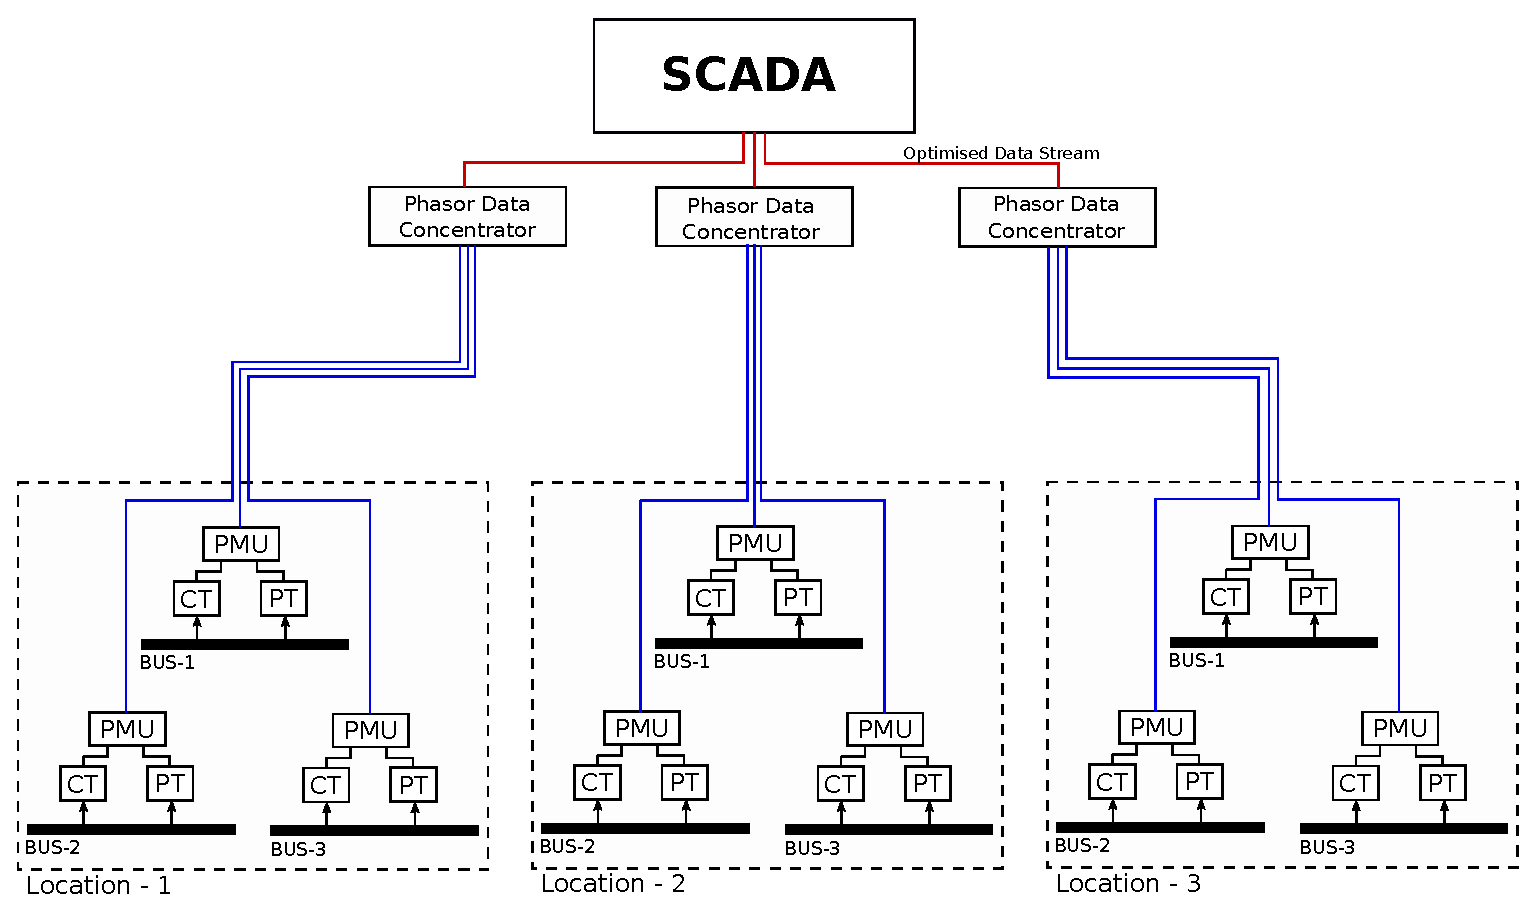
\includegraphics[width=\textwidth]{fig/wams.eps}
	\caption{Simplified structure of WAMS}
	\label{fig:wams}
\end{figure}

Fig. \ref{fig:wams} Shows a simplified architecture of modern Wide Area Measurement System. PMUs are installed at different substations on HV buses, via CTs and PTs, each PMU has multiple channels sampling AC waves at high rate. Rate of sampling varies according to the manufacturer and implementation of the scheme. Each PMU is provided a GPS receiver for accurate time with accuracy of approx 500 600 ns which is necessary for achieving time accuracy of 1-2 $\mu$s demanded by the standard. Each data after being sampled is then filtered using different DFT/FFT algorithm and is timestamped. This time stamped data is then sent to either SCADA or to a local Phasor Data Concentrator, which consolidates the data stream coming from different PMUs and send an bandwidth optimized data stream to the higher PDC or SCADA. 

\section{IEEE C37.118 Standard}

\subsection{Need of the standard}
This standard is for synchrophasor measurement, it defines synchronised phasor and frequency measurement is substation alng with requirements for measurement verification. Role of this standard is that measurements taken complient with and abiding to this standard will be readily accurately usable for power system analysis purposes. Standard achieves this by stating minimum necessary performance requirements of time-tagging, sampling and communication requirements to which a PMU has to adhere.

IEEE 1344-1995 is the original standard which was succeeded by IEEE C37.118-2005. 2005 standard mostly followed equipment manufacturers and the system integrators and was stating performance of steady-state conditions. After the advancements and development in fault analysis dynamic synchrophasors were being used for the control and analysis.  which was the major reason of Revision-2011, which was immediately followed by revision 2014 which simplified the stringent norms laid down by it's predecessor.

\subsection{Definations, acronyms and abbriviations}

Before diving in to details lets clear out few useful terminologies for ease of understanding and appreciation of the subject:\\
\textbf{Phasor:} A complex equivalent of a sinusoidal wave quantity such that the complex modulus is the cosine wave amplitude, and the complex angle (in polar form) is the cosine wave phase angle.\\
\textbf{UTC:} Its is the time of day at the earth's prime meridian.\\
\textbf{ROCOF:} It is the measure at which the frequency changes in a given instance of time.\\
\textbf{Rate of change of Frequency Error (RFE):} The measure of error between the theoretical ROCOF and the measured ROCOF for the given instant of time.\\
\textbf{Frame:} A data frame or a frame of data is a set of synchrophasor, frequency, and ROCOF measurements that corresponds to the same time stamp.\\
\textbf{Anti-aliasing:}The process of filtering a signal before sampling to remove components of that signal whose frequency is equal to or greater than the Nyquist frequency (one-half the sample rate). If not removed, these signal components would appear as a lower frequency component (an alias).\\
\textbf{Nyquist frequency:} A frequency that is one-half the sampling frequency of a discrete signal processing
system.\\

\subsection{Requirements and Compliance}
Just like all other engineering devices PMU's reliability, accuracy  and precision are very crucial for its application and hence different kinds of test are done to validate its performance. Hence just like other measuring devices PMU standards are defined which states minimum performance requirement(s). All device should at least meet the requirement stated by the standards, according their application.


\subsubsection{Total Vector Error}
Classically error is the deviation of the measurement from the ideal quantity. It is computed from the difference between the Actual to the measured value. In case of synchrophasors the comparison involves difference in both amplitude and angle which are time dependent making the task even tougher. these quantities are considered combinely in the standards and is called "Total Vector Error (TVE)" \cite{c37.118}.  

TVE is an expression of the difference between a ``perfect" sample of a theoretical synchrophasor and the estimate given by the unit under test at the same instant of time. The value is normalized and expressed in per unit of the theoretical phasor. Which can be mathematically represented as: 
\begin{equation}
TVE(n) = \sqrt{\frac{ (\hat{X}_r(n) - X_r(n))^2 + (\hat{X}_i(n)-X_i(n))^2} {X_r(n)^2 + X_i(n)^2}}
\end{equation}
Here $ \hat{X}_r (n)$ and $\hat{X}_i(n) $ are the estimated values of the given phasor and $X_r$ and $X_i$ are the theoretical values.
To be complient with standard, PMU shall provide synchrophasor, frequency, and ROCOF measurements that meet the requirements as per the standards at a given time instance \textit{n}. Similarly for freq and ROCOF the validation will be done using following equations:
\begin{eqnarray}
FE == |f_{true}-f_{measured}| = |\Delta f_{true}-\Delta f_{measured}| \\
RFE == |(df/dt)_{true}-(df/dt)_{measured} |
\end{eqnarray}

\subsubsection{Class of PMU:}
Depending up on the application PMU are classified in two types and depending upon the class their error tolerance is evaluated, there are two classes:
\begin{enumerate}
	\item \textbf{Measurement Class (M):} As the name suggests these are used for measurement and instrumentation purposes. These PMUs are intended for slower response time and greater precision. These kind of PMUs are used for analytical purposes and hence often do not require minimal (reporting) delay or fastest reporting speed.
	\item \textbf{Protection Class (P):} These PMUs are designed for fastest responses time. They may have (slightly) inferior reporting precision and soft-realtime operation. 
	mandates no explicit filtering
\end{enumerate} 

\subsubsection{Validation \& Testing }

To get the TVE, compliance tests are performed and during the test only the quantity under test is varied from the reference condition as per the test and other relevant quantities are maintained at reference condition. There are following kind of compliance tests:
\begin{enumerate}
	\item Steady-state compliance
	\begin{enumerate}
		\item Steady-state synchrophasor measurement requirements
		\item Steady-state frequency and ROCOF measurement requirements
	\end{enumerate}
	\item Dynamic compliance
	\begin{enumerate}
		\item Synchrophasor measurement bandwidth requirements using modulated test signals
		\item Ramp of system frequency
		\item Step changes in phase and magnitude
	\end{enumerate}
\end{enumerate} 
The TVE tolerance for each case wont be mentioned here as those tables can be looked into the standards.


\subsubsection{Time Synchronization}

The PMU should be capable of receiving time from a reliable and accurate source such as GPS that can provide time traceable to UTC with sufficient accuracy for calculating Total Vector Error (TVE), Frequency Error and rate of change of frequency error (RFE), all measurements are synchronized to UTC.
This is a vital parameter because time error of 1$\mu$s would result in to 0.022 degree and 0.018 degree in 60 Hz and 50 Hz systems respectively. And a phase error of 0.57$\deg$ will result in to 1\% TVE. This corresponds to error tolerance of $\pm26 ~\mu$s for 60 Hz and $\pm 31 ~\mu s$ for 50 Hz system.

\subsubsection{Reporting Rate}
Estimate of synchrophasor, Frequency and ROCOF will be made so that they can be reported to data concentrator and the reporting rate should be constant i.e. the time difference between two reports received from a PMU should be same. This reporting rate will be integer number of times per second and should be in integer multiple of the of the power nominal-frequency. Hence required rate of reporting as mentioned below:

\begin{table}
	\begin{center}
		\setlength\arrayrulewidth{1pt}
		\begin{tabular}{|c|c|c|c|c|c|c|c|c|c|}
			\hline
			System Frequency & \multicolumn{3}{c}{50 Hz} & \multicolumn{6}{|c|}{60 Hz}\\
			\hline 
			Reporting Rate (Fs)& 10 & 25 & 50 & 	10& 12 &15 & 20 & 30 & 60\\
			\hline
		\end{tabular}
	\end{center}
\end{table}
 

\subsubsection{Performance Parameters}
These are the parameters considered as qualitative factors to judge the PMU performance. 

\begin{itemize}
	\item  \textit{Measurement response time:} Measurement response time is the time to transition between two steady-state measurements before and
	after a step change is applied to the input. This is measured by applying a step change in amplitude or phase and holding the input constant otherwise and measuring the time taken  by the PMU to settle to a steady-state value. response time is determined from the accuracy evaluation of the measurements, not step time or the stepped	parameters themselves.
	\item \textit{Measurement delay time:} It is the time difference between the step input applied and the measurement time that the output reaches 50\% of the final or steady state value.  
	\item \textit{Measurement Reporting Latency:} Reporting Latency is the time lag between the event occurs in the power system and it is reported in the data. It is one of the important quantitative and qualitative parameter, as it depends on al most all factors involved like sample window, filter delay, processing time, processor speed etc. Here reporting rate and PMU class play major role in deciding the delay. 
	\item \textit{Measurement and operational errors:} It is a self-health-test flag. as per standard PMU should send a status flag with each measurement stating the error at PMU end. this error bit can incorporate issue in any aspect(s) like ADC error, memory over flow, etc.
\end{itemize}

\subsubsection{Communication Compliance}
